\section{Descrição do problema}

The size of offshore lifts can be reduced by making the construction modular,
with each module being constructed onshore and then lifted using a crane vessel 
into place onto the platform. A number of very large crane vessels were built in 
the 1970s which allow very large single modules weighing up to 14,000 tonnes to 
be fabricated and then lifted into place.

\begin{figure}[h!]
    \centering
    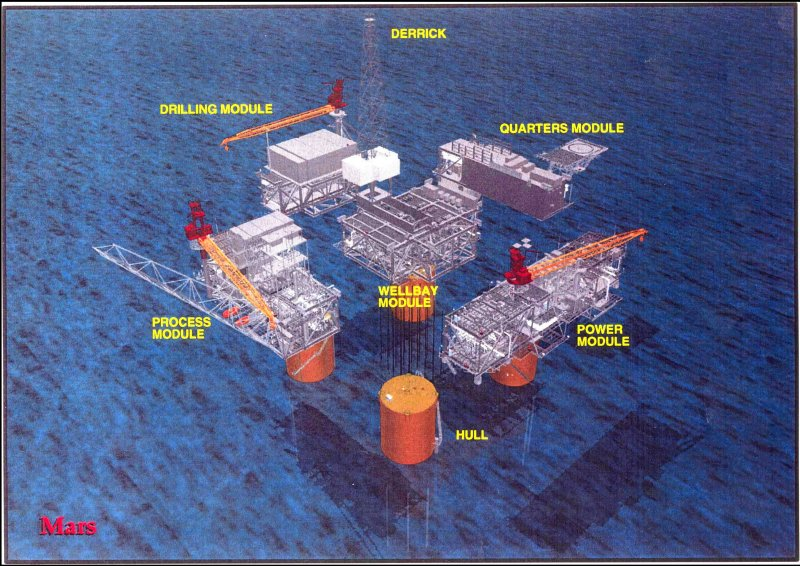
\includegraphics[width=0.9\columnwidth]{figs/mating/modules}
    \caption{Módulos de uma plataforma.}
    \label{modulos}
\end{figure}

\begin{figure}[h!]
    \centering
    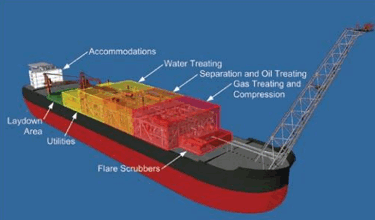
\includegraphics[width=0.9\columnwidth]{figs/mating/fpso_modules}
    \caption{Módulos em um FPSO.}
    \label{fpso_modulos}
\end{figure}

 mating (processo de acoplamento entre módulos e casco)

P-55 Platform
The deck mating procedure entailed lifting the deckbox, a technique never used
before in Brazil

This is the first time a deck mating operation, coupling the modules and hull,
has ever been done using this technique. The deckbox, weighing 17,000 tonnes, 
was raised over 40 meters and lowered onto the hull. The usual procedure is to 
lower the hull. The P-55 and the eight replicant FPSOs to be built here will be 
Brazilian and international benchmarks.

Isso possibilitou a construção simultanea dos dois módulos

Na operação, o convés (deck box) da plataforma, uma estrutura de 17 mil
toneladas, foi içado a uma altura de 45 metros e acoplado ao casco, parte inferior da plataforma.

\href{http://www.offshoreenergytoday.com/brazils-petrobras-completes-deck-mating-on-p-55-platform/}{P-55\textit{Deck
Mating}}

\begin{figure}[h!]
    \centering
    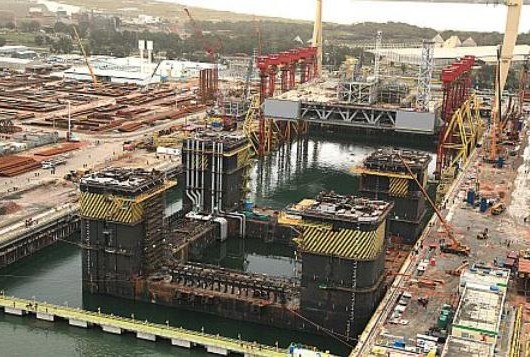
\includegraphics[width=0.9\columnwidth]{figs/mating/P55}
    \caption{Alinhamento da plataforma P-55.}
    \label{P55}
\end{figure} 

Durante a execução da P-53, já montada pela Quip no mesmo local, o içamento de
alguns módulos foi feito com uso de guindastes flutuantes, o que exigia paralisações 
na movimentação de navios na área do Porto Novo. De acordo com o gestor
executivo da Quip, essa interferência não ocorrerá na integração dos módulos da P-63, 
pois não serão utilizados guindastes flutuantes. Desta vez, para o içamento dos módulos 
e instalação deles no casco da plataforma, será utilizado um guindaste de grande porte 
fixo em terra, com capacidade para içar até 3,5 mil toneladas. Este equipamento terá como 
apoio uma base de concreto de 90 metros de largura por 90 metros de comprimento, a ser construída 
no cais. 

A P-63 é uma plataforma do tipo FPSO (Floating Production Storage and
Offloading). Terá capacidade para processar 140 mil barris por dia de 
petróleo e 1 milhão de Nm³/dia de compressão de gás. A unidade gerará 
98 Mwh de energia e armazenará até 1,4 milhão de barris de petróleo. 
No pico de sua construção, deverão ser gerados em torno de 2 mil empregos 
diretos.

Embraer ITA - Automatic alignment and levering process for aircraft fuselage
using anthropomorphic robots assisted by external measurement systems, such
as iGPS, Laser Radar, laser tracker, optical systems and theodolites 

Tecnhnipipe - used the Laser Scanner to perform a preparatory study for 
the installation of a crane on a town centre site. One of its clients, 
a civil engineering company, planned to erect a crane there and wanted 
to study the available space with respect to the span and height of the 
crane. In a town centre, particularly because of safety restrictions, the rotation of the crane is limited by the buildings that surround the site. For this reason, the positions of the ridges of the surrounding buildings, the trees and the electricity poles must be known and mapped to determine the points where the crane should be fixed
